 \chapter{Numerical results for the implicit coupling schemes}

This chapter provides validation and comparison results for the implicit solution schemes.
It focuses on two examples.

\section{Second Danilovskaya problem}

The second Danilovskaya problem is proposed in \cite{danilovskaya_dynamical_1952} and it is used frequently in the literature for the validation of a fully coupled thermomechanical model (\cite{farhat_unconditionally_1991}, \cite{tosaka_boundary_1991}, \cite{tamma_effective_1992}, \cite{tanaka_application_1995} and \cite{danowski_computational_2014}).
Following the description in \cite{danowski_computational_2014}, the geometry is in the form of a cuboid of height and width equal to \SI{4}{\milli\meter} and a length of \SI{6}{\milli\meter}, as is shown in Figure~\ref{fig:setup_2nd_danilovskaya}.
The solid is linear elastic and subject to a heat flux on the surface \(x=\SI{0}{\milli\meter}\).
Here, \(\hat Q_C \equiv \hat q_C\) \jvc{Make notation consistent.} as only small deformation, i.e., \(\mathbf F \equiv \mathbf I\), are considered.

\begin{figure}
  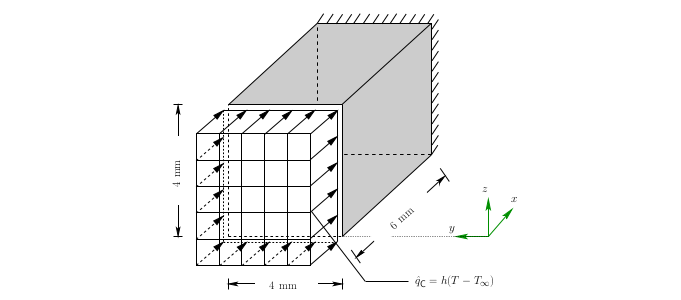
\includegraphics[width=\textwidth]{figures/setup_2nd_danilovskaya.png}
  \caption{Setup for the second Danilovskaya problem. Initial geometry and prescirbed heat convection boundary condition \(\hat q_C\).}
  \label{fig:setup_2nd_danilovskaya}
\end{figure}

The simulation performed in three spatial dimensions.
However, all displacement degrees of freedom in the \(y\)- and \(z\)-directions are fixed, such that a quasi-one-dimensional motion is produced.
The body is assumed to be mechanically constrained and thermally insulated.

The mechanical and thermal field properties are given in Table~\ref{tab:snd_danilovskaya_description}, where \(\bar{h}\) denotes the kinematic heat transfer coefficient, defined as \(\bar{h}=\frac{h}{\rho C_V}\) with the linear heat transfer coefficient \(h\).
Furthermore, the values for the thermal conductivity \(k\), the coefficient of thermal expansion \(\alpha_{T}\), the constant initial temperature \(T_{0}\), as well as an ambient temperature \(T_{\infty}\) are given.
The elastic constants characterizing the material are the Young's modulus \(E\) and Poisson's rate \(v\).
A linear thermoelastic material is chosen according to the model described in \cite{armero_new_1992}.

In the literature (\cite{farhat_unconditionally_1991}, \cite{tosaka_boundary_1991}, \cite{tamma_effective_1992}, \cite{tanaka_application_1995}), the density \(\rho\) and the heat capacity \(C_V\) are not divulged, and can in theory, be chosen arbitrarily according a dimensionless termomechanical parameter \(\delta\).
However, to achieve a direct comparison with the results in \cite{tanaka_application_1995}, \cite{danowski_computational_2014} chose after calibration \(\rho=\SI{7.850}{\kilo\gram\meter^{-3}}\), yielding \(C_V = \SI[exponent-mode=engineering]{0.821}{\joule\kg^{-1}\kelvin^{-1}}\).
These values are adopted here as well.

\begin{table}
  \centering
  \caption{Material properties, and initial and boundary conditions for the second Danilovskaya problem.}
  \label{tab:snd_danilovskaya_description}
  \begin{tabular}{ccS[exponent-mode=engineering]}
  \multicolumn{2}{c}{Material Properties} & {\vphantom{\Big |}Effective value}\\
  \hline\hline
  \vphantom{\Big |}Density \(\rho\) & (\si{\newton\second^2\milli\meter^{-4}}) & 7850e-12\\
  \vphantom{\Big |}Young's modulus \(E\) & (\si{\newton\milli\meter^{-2}}) & 210e3\\
  \vphantom{\Big |}Poisson's coefficient \(\nu\) & - & 0.3\\
  \vphantom{\Big |}Conductivity \(k\) & (\si{\newton\second^{-1}\kelvin^{-1}}) & 1.03\\
  \vphantom{\Big |}Heat capacity \(C_V\) & (\si{\milli\meter^2\second^{-2}\kelvin^{-1}}) & 0.821e6\\
  \vphantom{\Big |}\makecell[c]{Coefficient of\\ thermal expansion} \(\alpha_T\) & (\si{\kelvin^{-1}}) & 1.1e-6\\
  \hline
  \multicolumn{2}{c}{Boundary Conditions\vphantom{\Big |}} & \\\hline
  \vphantom{\Big |}Dimension \(l_x\) & (\si{\milli\meter}) & 6\\
  \vphantom{\Big |}Dimension \(l_y\) & (\si{\milli\meter}) & 4\\
  \vphantom{\Big |}Dimension \(l_z\) & (\si{\milli\meter}) & 4\\
  \makecell[c]{Kinetic heat\\ convection coefficient} \(\bar h\) & (\si{\milli\meter\second^{-1}}) & 100e-3\\
  \multicolumn{3}{c}{\vphantom{\Big |}All mechanical degrees of freedom fixed in the \(y\)- and \(z\)-directions.}\\
  \hline
  \multicolumn{2}{c}{Initial Conditions\vphantom{\Big |}} & \\\hline
  \vphantom{\Big |}Ambient temperature \(T_\text{env}\) & (\si{\kelvin}) & {373.15}\\
  Intial temperature \(T_0\) & (\si{\kelvin}) & {273.15}\\
  \hline
  \multicolumn{2}{c}{Reference value \vphantom{\Big |}} & \\\hline
  \vphantom{\Big |}Temperature at point \(E\) (\(x=\SI{1}{\milli\meter}\)) & (\si{\kelvin}) & \\
  \hline\hline
  \end{tabular}
\end{table}

The discretisation for both the mechanical and thermal field contains each \(n_{x} \times n_{y} \times n_{z}=12 \times\) \(4 \times 4\) Hex 8 elements.
The simulation time is \(t=\SI{4}{\second}\), with a time-step size of \(\Delta t=\SI{0.001}{\second}\).
Moreover, a one-step- \(\theta\) time integration is chosen with the value \(\theta=0.5\), resulting in a CrankNicolson scheme for the temperature field, and quasi-static approach for the mechanical field.
Displacements and temperatures are evaluated at the centre point of the plane at \(x=\SI{1}{\milli\meter}\).

\section{Expansion of a thermoelastic thick-walled cylinder}

The example of quasi-static finite strain thermo-elastic expansion of an infinite long thick-walled cylinder was introduced in [10] and studied again in [25,33].
In this paper we want to compute this example again using exactly the same geometrical set-up and the same material properties.
In contrast to these papers, where the axis symmetric cylinder was meshed by ten iso-parametric 4-node quadrilateral elements, the problem is discretized in this paper with three-dimensional high-order hexahedral solid elements with a polynomial degree of \(p=5\); see Fig. 11. \jvc{Describe our FEM discretization}
The same discretization and polynomial degree is used for both subproblems. Thanks to its symmetric structure, only one-fourth of the cylinder is considered with an inner radius of \(r_{0}=10 \mathrm{~mm}\) and an outer radius of \(r_{1}=20 \mathrm{~mm}\), as depicted in Fig. 10.
All material properties and model properties can be found in Table \(2\).

\begin{table}
  \centering
  \caption{Material properties, and initial and boundary conditions for the problem concerning the expansion of a thick-walled cylinder.}
  \label{tab:snd_danilovskaya_description}
  \begin{tabular}{ccS[exponent-mode=engineering]}
  \multicolumn{2}{c}{Material Properties} & {\vphantom{\Big |}Effective value}\\
  \hline\hline
  \vphantom{\Big |}Density \(\rho\) & (\si{\newton\second^2\milli\meter^{-4}}) & 7.8e-9\\
  \vphantom{\Big |}Bulk modulus \(\kappa\) & (\si{\newton\milli\meter^{-2}}) & 164206\\
  \vphantom{\Big |}Shear modulus \(\mu\) & (\si{\newton\milli\meter^{-2}}) & 80194\\
  \vphantom{\Big |}Conductivity \(k\) & (\si{\newton\second^{-1}\kelvin^{-1}}) & 45\\
  \vphantom{\Big |}Heat capacity \(C_V\) & (\si{\milli\meter^2\second^{-2}\kelvin^{-1}}) & 460e6\\
  \vphantom{\Big |}\makecell[c]{Coefficient of\\ thermal expansion} \(\alpha_T\) & (\si{\kelvin^{-1}}) & {\SI[exponent-mode=engineering]{2e-5}{} - \SI[exponent-mode=engineering]{1.5e-4}{}}\\
  \hline
  \multicolumn{2}{c}{Boundary Conditions\vphantom{\Big |}} & \\\hline
  \vphantom{\Big |}Inner radius \(r_0\) & (\si{\milli\meter}) & 10\\
  \vphantom{\Big |}Outter radius \(r_1\) & (\si{\milli\meter}) & 20\\
  \vphantom{\Big |}Inner radius rate of displacement \(\dot u_1\) & (\si{\milli\meter\second^{-1}}) & 1\\
  \vphantom{\Big |}Heat at inner radius \(q_1\) & (\si{\newton\second^{-1}\milli\meter^{-1}}) & 0\\
  \vphantom{\Big |}Temperature outter radius \(\theta_1\) & (\si{\kelvin}) & 273.15\\
  % \multicolumn{3}{c}{\vphantom{\Big |}All mechanical degrees of freedom fixed in the \(y\)- and \(z\)-directions.}\\
  \hline
  \multicolumn{2}{c}{Initial Conditions\vphantom{\Big |}} & \\\hline
  Intial temperature \(T_0\) & (\si{\kelvin}) & {273.15}\\
  \hline
  \multicolumn{2}{c}{Reference value \vphantom{\Big |}} & \\\hline
  \vphantom{\Big |}Temperature at inner radies (\(r=r_0\)) & (\si{\kelvin}) & \\
  \hline\hline
  \end{tabular}
\end{table}

On the front and reverse surface, the displacement boundary conditions are restricted to zero \(u_{z}=0\).
Nor does any heat transfer takes place, i.e. the heat flux is zero.
Furthermore, zero heat flux is also imposed at the inner radius, whereas the reference temperature \(\Theta_{0}\) is imposed on the outer radius.
A displacement driven computation is chosen by increasing the imposed displacement at the inner radius with a constant displacement rate of \(\dot{u}_{0}\).
Following [10], the maximum displacement is set to three times of the wall thickness until \(u_{\max }=30 \mathrm{~mm}\) is reached, which clearly involves large deformations.

In accordance with [10] we choose the following decoupled Neo-Hookean free energy function
\[
\hat{\Psi}=\hat{\mathrm{U}}(\mathrm{J})+\hat{\mathrm{W}}(\overline{\mathbf{C}})+\hat{\Psi}_{\Theta}(\Theta)+\hat{M}(\mathrm{~J}, \Theta)
\]
where the volumetric \(\hat{U}(J)\) and the isochoric \(\hat{W}(\overline{\mathbf{C}})\) part yield
\[
\hat{\mathrm{U}}(\mathrm{J})=\frac{\kappa}{2} \ln ^{2}(\mathrm{~J}), \quad \hat{\mathrm{W}}(\overline{\mathbf{C}})=\frac{\mu}{2}[\operatorname{tr}(\overline{\mathbf{C}})-3] .
\]
In addition, we choose for the thermal part
\[
\hat{\Psi}_{\Theta}(\Theta)=c\left[\left(\Theta-\Theta_{0}\right)-\Theta \ln \left(\Theta / \Theta_{0}\right)\right]
\]
resulting in a constant specific heat capacity \(c_{p}=c\) and finally assume a coupled part as
\[
\hat{M}(J, \Theta)=-3 \alpha\left(\Theta-\Theta_{0}\right) \frac{d \hat{U}(J)}{d J}=-3 \alpha \kappa\left(\Theta-\Theta_{0}\right) \frac{\ln (J)}{J}
\]
which models the assumption of purely volumetric thermal expansion; see [7]. The coupled part \(\hat{M}(\mathrm{~J}, \Theta)\) represents the thermo-mechanical coupling effects since the volumetric stress tensor reads
\[
\mathbf{S}_{\mathrm{vol}}(\mathbf{C}, \Theta)=\mathrm{Jp} \mathbf{C}^{-1}=\kappa\left[\ln J-3 \alpha\left(\Theta-\Theta_{0}\right) \frac{(1-\ln \mathrm{J})}{\mathrm{J}}\right] \mathbf{C}^{-1}
\]
where \(p=\mathrm{d} \hat{\Psi} / \mathrm{dJ}\) and the thermo-elastic coupling follows from (17):
\[
\mathscr{H}(\mathbf{C}, \Theta)=\Theta \frac{\partial^{2} \Psi}{\partial \mathrm{J} \partial \Theta} \mathrm{J}=-3 \alpha \kappa \Theta \frac{(1-\ln \mathrm{J})}{\mathrm{J}^{2}} \mathrm{~J}
\]
All upcoming numerical simulations were performed with the same material whose parameters are summarized in Table 2 .

\subsection{Weak coupling}


\begin{figure}
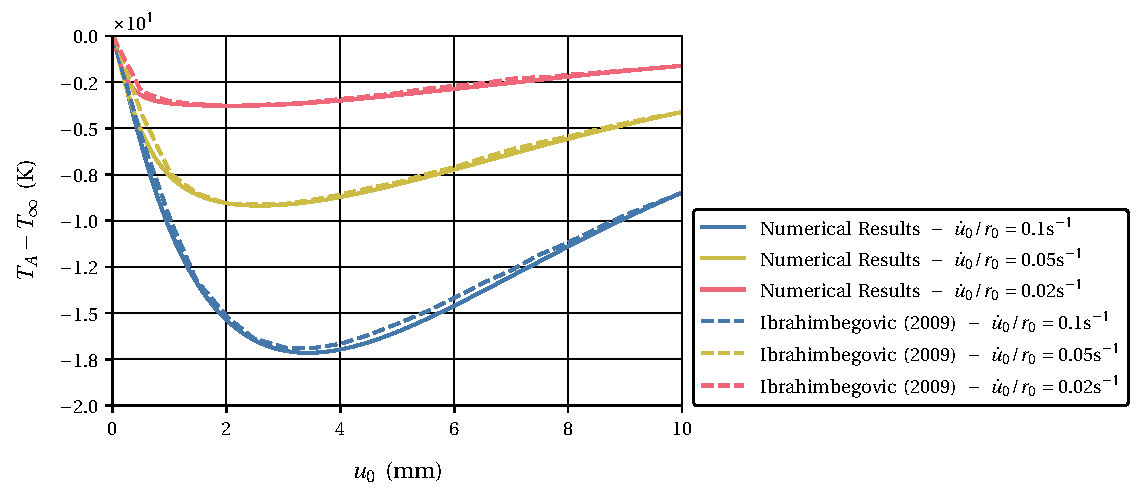
\includegraphics[width=\textwidth]{val_weak_coupling_ibra_inner_radius_temperature_coupled_quad4fbar}
\end{figure}


\subsection{Strong coupling}

\subsubsection{Methods with only one residual evaluation per iteration}

\subsection{Newton-GMRES method}

\subsection{Broyden-like method}

\subsection{Polynomial vector extrapolation with cycling}\jvc{Check if the name is not the other way around}

\subsection{Comparison for the best methods}

\begin{figure}
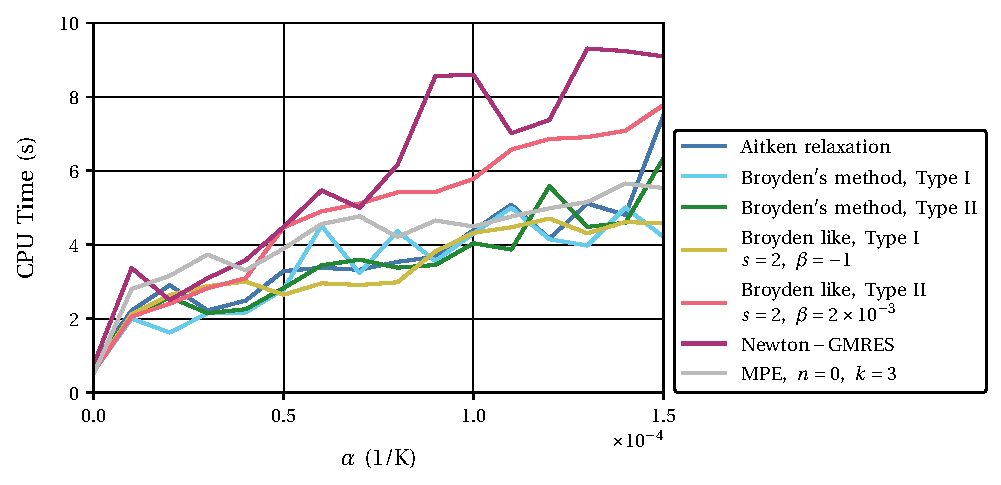
\includegraphics[width=\textwidth]{thick_cylinder_comparison_methods_best_cpu_time_coupl_strength_quad4fbar_pred}
\end{figure}

\begin{figure}
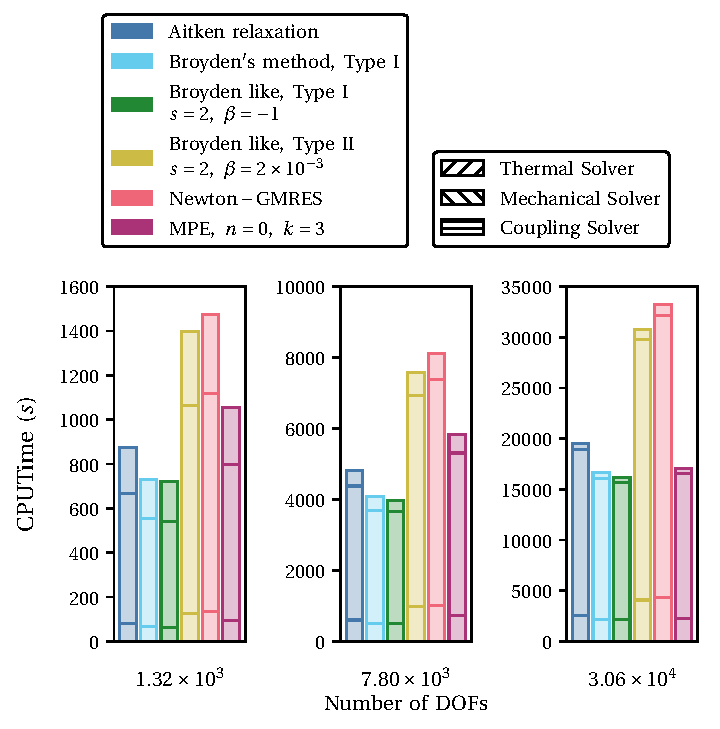
\includegraphics[width=\textwidth]{thick_cylinder_comparison_methods_best_time_profile_mesh_size_quad4fbar_pred}
\end{figure}

% \begin{table}
%   \centering
%   \caption{Material properties, and initial and boundary conditions for the problem concerning the expansion of a thick-walled cylinder.}
%   \label{tab:snd_danilovskaya_description}
%   \begin{tabular}{c
%     S[exponent-mode=engineering]
%     S[exponent-mode=engineering]
%     S[exponent-mode=engineering]
%     S[exponent-mode=engineering]
%     S[exponent-mode=engineering]
%     S[exponent-mode=engineering]}
%   $\Delta t$ \si{\second} & {\multicolumn{3}{c}{0.1}} & {\multicolumn{3}{c}{1.0}}\\
%   $\alpha$ \SI{1e-5}{\kelvin^{-1}} & {5} & {10} & {15} & {5} & {10} & {15}\\
%   \hline\hline
%   \hline\hline
%   \end{tabular}
% \end{table}

\section{Necking}

\begin{figure}
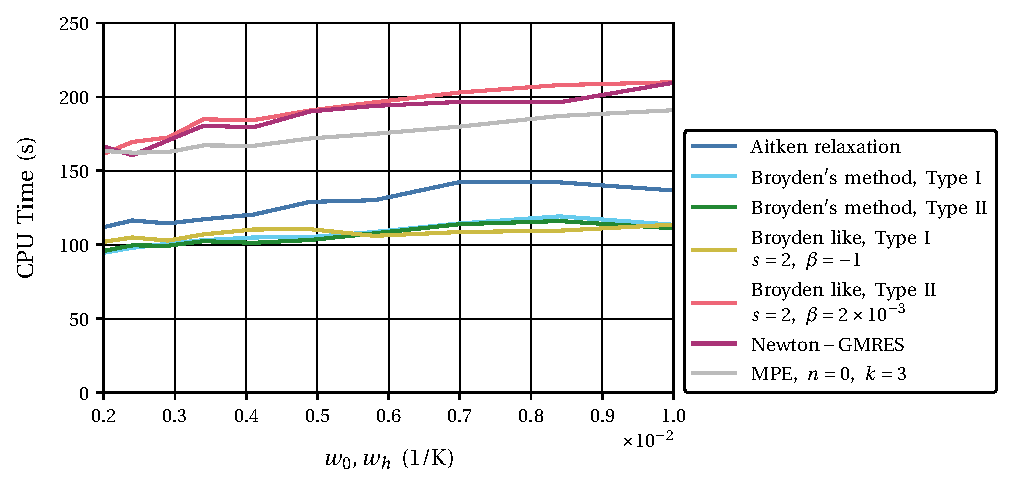
\includegraphics[width=\textwidth]{necking_comparison_methods_best_cpu_time_coupl_strength_quad4fbar_pred}
\end{figure}

\begin{figure}
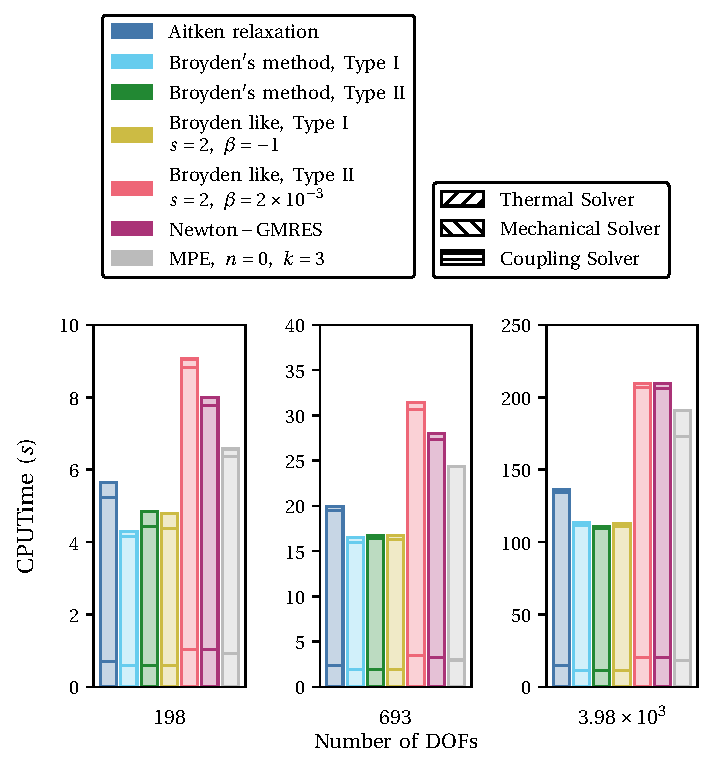
\includegraphics[width=\textwidth]{necking_comparison_methods_best_time_profile_mesh_size_quad4fbar_pred}
\end{figure}
